\documentclass[12pt]{report}
\usepackage{amssymb,amsmath,latexsym}
\usepackage[framed,numbered,autolinebreaks,useliterate]{mcode}
\usepackage{graphicx}
\usepackage{subcaption}
\usepackage[export]{adjustbox}
% Page length commands go here in the preamble
\setlength{\oddsidemargin}{-0.25in} % Left margin of 1 in + 0 in = 1 in
\setlength{\textwidth}{7in}   % Right margin of 8.5 in - 1 in - 6.5 in = 1 in
\setlength{\topmargin}{-.75in}  % Top margin of 2 in -0.75 in = 1 in
\setlength{\textheight}{9.2in}  % Lower margin of 11 in - 9 in - 1 in = 1 in

\newtheorem{theorem}{Theorem}
\newtheorem{definition}{Definition}

\renewcommand{\baselinestretch}{1.5} % 1.5 denotes double spacing. Changing it will change the spacing
\setlength{\parindent}{0in} 
\begin{document}
\title{Plasma Physics Term Project:
\\
 Atmospheric Re-entry Problem}
\author{Anil Aksu}
\date{\today}
\maketitle
\abstract{This document explains how the state quantities such as temperature and pressure field and electric field are affected by the shock surface in atmospheric re-entry problem. It is done under continuum assumption, therefore magneto-hydrodynamic is used. Moreover, as a benchmark solution, the compressible 1-D flow is solved. Finally, it is found that the presence dramatically affect temperature and electric field.}
\tableofcontents
\listoffigures
\newpage
\chapter{Introduction}
The earth is surrounded by so-called atmosphere which creates a sufficient environment to form living organisms on planet in many ways. One particular way that atmosphere protects the earth  is to shield solar winds magnetically. However, this leads to accumulation of charged particles within a certain layer of atmosphere \cite{Chen}. In detail, the atmosphere consists of 6 layers which are Troposphere, Stratosphere, Mesosphere, Ionosphere, Thermosphere and Exosphere\cite{NetAtm}:  

\begin{itemize}
   \item \emph{ \color{blue} Troposphere:} {\small The troposphere is the lowest part of the atmosphere and  also where almost all weather takes place.} 
   \item \emph{ \color{blue} Stratosphere:} {\small The second region of atmosphere extending upward from the tropopause characterized by vertical gradient in temperature which triggers internal waves within Stratosphere. }
   \item \emph{ \color{blue} Mesosphere:} {\small The mesosphere is directly above the stratosphere. Temperature decreases with height throughout the mesosphere with minimum $183K$.}
   \item \emph{ \color{blue}Ionosphere:} {\small The layer of atmosphere that is ionized by solar and cosmic radiation with temperature cycles within $200K$-$500K$.}
   \item \emph{ \color{blue} Thermosphere:}{\small The region of the atmosphere where a continuous medium assumption fails.}
   \item \emph{ \color{blue} Exosphere:}{\small The uppermost layer, where the atmosphere diminishes and merges with interplanetary space.}
   \end{itemize}
In the particular problem we are interested in, the primary attention is paid to ionosphere where the most critical physical changes occur within the atmosphere during re-entry of a rocket. Inside ionosphere, during diurnal cycle, the solar flux shows significant variation\cite{Chen} which seriously changes the dynamics of the re-entry problem. The solar flux affects the conditions in terms of both ionization and temperature which are both critically important. The degree of ionization will determine the total drag force applied to the rocket induced by electromagnetic forces. As the degree of ionization increases the electromagnetic forces become more pronounced. Moreover, the increase in temperature will substantially determine flow conditions. As the speed of sound is directly dependent on temperature as follows:
\begin{equation}
\label{eq:1}
c=\sqrt{\gamma R T}.
\end{equation}
where $\gamma$ is gas constant and $R$ is Boltzmann constant. The temperature will determine if the rocket velocity is supersonic or subsonic. If the velocity of the rocket $V>c$, then it is supersonic flow, but if $V<c$, it is subsonic flow. The presence of shock seriously affects the state quantities like temperature, pressure, density before and after a shock. These quantities become important in terms of drag calculations also the thermal design of a rocket. 
\begin{figure}
\label{fig:Atmosphere}
  \centering
      \includegraphics[scale=0.3]{AtmosphereLayers.png}
      \caption{Layers of Atmosphere shown schematically.}
\end{figure}
In case of ionospheric re-entry, electromagnetic quantities like electric field and magnetic field\cite{Savino,Votta} are affected by the presence of a shock. Understanding of electromagnetic effects may both help to improve the thermal and mechanical design of a rocket or a space vehicle but also may allow to control the plasma flow field remotely to reduce the disruptive effects.

\begin{figure}
\label{fig:rocket}
  \centering
      \includegraphics[scale=0.2]{Rocket.png}
  \caption{Re-entry Rocket with representative shocks which create sharp changes in pressure, velocity and density fields.}
\end{figure}
\section{Plasma Flows}
Plasma is commonly referred as the forth state of matter which is generally obtained at high temperatures\cite{IntPlasma}. Differing from classical compressible gas dynamics, electromagnetic effects are also effective in plasma flows. It is modelled either as continuum or statistically. The continuum model assumes the mean free path between particles are smaller than the mechanistic effects. This means spatial dimension of a continuum motion where usually a problem specific length scale is defined, is much bigger than mean free path of particles. 
\\
This approach leads to magneto-hydrodynamic models which are classified by the number of species present in the flow field\cite{IntPlasma}. These species are ions and  electrons, however there may be more than one type of ion. In magneto-hydrodynamic (MHD) models, there are separate continuity, momentum and energy equations for each species, but they are coupled by interaction forces between each species. Furthermore, even though there are more than one species, the electromagnetic forces are modelled by Maxwell's equations for all species not separately\cite{IntPlasma,Vasilevski}. In this present study, these equations are used and they are given in more detail in the analysis chapter.
\\
Furthermore, the statistical model assumes that ionized particles, electrons and ions, have thermal property such that it obeys statistical distribution such as Maxwellian. Its integral within a particular volume and velocity distribution gives the amount of particle within a given volume. 
\begin{equation}
	n_i=\int_V\int_{-\infty}^{\infty}f_i(\mathbf{x},\mathbf{v},t)\mathrm{d}\mathbf{v}\mathrm{d}\mathbf{x}.
\end{equation}
The distribution above is given for ions. Similar distribution can be employed for electrons as well, therefore,
\begin{equation}
n_e=\int_V\int_{-\infty}^{\infty}f_e(\mathbf{x},\mathbf{v},t)\mathrm{d}\mathbf{v}\mathrm{d}\mathbf{x}.
\end{equation}
The distribution above evolves in time as follows:
\begin{equation}
\frac{\partial f}{\partial t}+ \mathbf{v}\frac{\partial f}{\partial x}+\frac{q\mathbf{E}}{m}\frac{\partial f}{\partial \mathbf{v}}=0.
\end{equation}
The electric field $\mathbf{E}$ can be formulated in terms of a potential field $\phi$.
\begin{equation}
\mathbf{E}=-\mathbf{\nabla}\phi.
\end{equation}
and also 
\begin{equation}
\epsilon_0 \mathbf{\nabla}^2 \phi=e(n_e-Zn_i).
\end{equation}
These are the governing equations of plasma flow. However, this is the simplest possible model which only considers the effect of electric field. But in most applications, the magnetic field is also effective\cite{IntPlasma}.
\subsection{Shocks In Plasma Flows}
 The shock waves are basically discontinuity in density $\rho$, velocity $\mathbf{u}$ and temperature $T$. These relations are obtained by mass continuity, momentum and energy equations. In the end, shock relations are obtained for all of them separately. First, the mass continuity is given as:
\begin{equation}
\frac{\partial \rho}{\partial t}+\frac{\partial \rho u}{\partial x}=0. 
\end{equation}
And also the momentum equation in 1-D without viscous effects is given as:
\begin{equation}
\label{eq:2}
\frac{\partial \rho u}{\partial t}+ \frac{\partial }{\partial x}\left ( \rho u^2 +p \right )=0,
\end{equation}
Finally the energy equation in 1-D is given as:
\begin{equation}
\label{eq:3}
\frac{\partial }{\partial t}\left ( \frac{1}{2}\rho u^2 + \rho e \right )+ \frac{\partial }{\partial x}\left ( \rho u(\frac{u^2}{2}+h)-\kappa \frac{\partial T}{\partial x} \right )=0.
\end{equation}
In addition to these governing equations, under the ideal gas assumption, the pressure can be related to the density and temperature as:
\begin{equation}
\label{eq:4}
p=\rho R T
\end{equation}
This formation is written in differential form, at the same time, these can be written in integral form by Green's theorem around infinitely thin shock surface given in figure 1.3. This analysis for the density jump can be given as:
\begin{equation}
\label{eq:5}
	\oint_{C} \rho u \mathrm{d} t-\rho \mathrm{d} x =0.
\end{equation}
 
\begin{figure}
\label{fig:shock}
\centering
\includegraphics[width=0.2\textwidth]{shock.png}
\caption{Shock Surface Illustration}
\end{figure}
Therefore, the closed integral can be written as:
\begin{equation}
\label{eq:6}
\oint_{N^+} \rho u \mathrm{d} t-\rho \mathrm{d} x-\oint_{N^-} \rho u \mathrm{d} t-\rho \mathrm{d} x =0.
\end{equation}
In the equation \ref{eq:1}, the closed curve is defined around the line of discontinuity with infinitely thin thickness. As usual, the closed integral formulation is in the counter-clockwise direction and $N^+$ denotes the line in higher dimensions surface before the shock wave and $N^-$ denotes the line in higher dimensions surface after the shock wave.
In generic form, the difference between the quantities $[f(\rho)]=f(\rho ^+)-f(\rho ^-)$ and $[\rho]=\rho ^+-\rho ^-$ are given in bracket notation. After replacing it in the equation \ref{eq:6}, it can be written as:
\begin{equation}
	[\rho]\mathrm{d} x=[ \rho u ]\mathrm{d} t.
\end{equation}
Furthermore, the similar shock formulation can be extended to momentum and energy equations, therefore three shock conditions are obtained. As mentioned earlier, the density, the pressure and
\newpage
the velocity field shows an abrupt change after a shock. An important non-dimensional parameter to characterize the flow is Mach number $M=U/c$ where $c$ is the speed of the sound given in equation \ref{eq:1}. 
\\
Recently, an analytical solution is obtained for 1-D compressible flow \cite{Johnson}, this will be used as benchmark case for the analysis of 2-D plasma shocks. The effect of electromagnetic forces on the location and the dynamics of a shock surface is not still well understood yet, there is considerable amount of applications where the shock surface are encountered in plasma flows such as atmospheric re-entry. In case of plasma flows, the abrupt changes observed in the density field and the temperature field may also be observed in the magnetic field and the electric field. After the shock surface, there is sudden decrease in the velocity field, therefore ionized particles accumulate in this region which also triggers an increase in electric field. As the electric field gets stronger, Lorentz force applied to charged particle also increases, this will change the structure of the shock surface.
\begin{figure}
\label{fig:shockflows}
\centering
\includegraphics[width=0.4\textwidth]{shockTS.jpg}
\caption{Supersonic to subsonic jumps in various types of flows.}
\end{figure}

\section{Problem Description And Objectives}
The shock formation in plasma flows is a complicated subject, because of this, the initial model is formulated in a simpler setting where we can compare our results with 1-D analytical model for compressible flow. Gaussian inlet profile with Mach number $M>1$ is given as boundary condition on the left boundary as shown in figure 1.5. Similar type of profile is also assigned to temperature field and ionized particle field. 
\\
In the absence of a obstacle, the flow field is supposed to show a self-similar profile, however in
\newpage
 the case we analyse here there is a rigid wall on the right boundary which stagnates the flow field, therefore it would lead to sudden change in the velocity field.  As a result, there will be a shock layer in front of the rigid wall. The location of the shock layer is compared with the analytical solution in 1-D\cite{Johnson}. The purposes of this comparison are first to find out if the numerical method gives reasonable results and secondly to understand how the presence of the electric field modifies this location. The effect of electric field will be controlled by controlling the charge density on the left boundary.
\begin{figure}
\label{fig:2DPlasmaDesc}
\centering
\includegraphics[width=0.8\textwidth]{2DPlasmaSurfaceInteraction.png}
\caption{Plasma Flow Configuration.}
\end{figure}
\\
Taking these into account, the objectives of the overall analysis can be summarized as:

\begin{itemize}
   \item {\small \emph{ \color{blue} Understanding the behaviour of shocks in Ionosphere:}}  How  the electric field induced by ions and electrons affect the shock surface.
   \item  {\small \emph{ \color{blue} How the presence of shock affects the electric field and the magnetic field:}}If there exist and abrupt change in the electric before and after shock layer.
   \end{itemize}
\chapter{Analysis}

\section{Magneto-hydrodynamic Model \label{MHD}}
In Magneto-hydrodynamic analysis, the plasma is treated as a single fluid \cite{IntPlasma}. Under this treatment, the density of the plasma is given as:
\begin{equation}
\label{eq:8}
\rho= n_i M +n_e m \approx n(M+m) \approx nM.
\end{equation}
where $n_i$ is the number of ions and $n_e$ is the number of electrons and also $M$ and $m$ are the masses of ions and electrons respectively. Moreover, the charge density is given as:
\begin{equation}
\label{eq:9}
\sigma = (n_i - n_e)e.
\end{equation}
Under this formulation, the single velocity in terms of ion and electron velocity can be given as:
\begin{equation}
\label{eq:10}
\mathbf{u}=(n_i M \mathbf{u}_i +  n_e m \mathbf{u}_e)\approx \mathbf{u}_i + (m/M)\mathbf{u}_e.
\end{equation}
As a start point single fluid magneto-hydrodynamic model\cite{IntPlasma} is used 
the continuity is given as:
\begin{equation}
\label{eq:12}
m_i\left [\frac{\partial n_i}{\partial t}+\frac{\partial n_i u_j  }{\partial x_j}\right ]=0. 
\end{equation}
If the continuity equation for ion and electron added, the continuity equation reduces to the following mass conservation equation:
\begin{equation}
\label{eq:13}
\frac{\partial \rho}{\partial t}+\mathbf{\nabla}\cdot \left ( \rho \mathbf{u} \right ) =0.
\end{equation}
This is well-known continuity equation in gas dynamics. Furthermore, the momentum equations for each species are given as\cite{hakimphd}:
\begin{equation}
\label{eq:14}
 \sum_{i} m_i n_i \left [\frac{\partial \rho \mathbf{u}_i}{\partial t}+ u_{i}^{j}\frac{\partial \mathbf{u}_i}{\partial x_j}    \right ]=-\mathbf{\nabla}p_i+n_i q_i \mathbf{E}+\mu \nabla^2 \mathbf{u}_i+R_{ik}(\mathbf{u}_k-\mathbf{u}_i),
\end{equation}
The equation \ref{eq:14} includes electric force and the interaction force $R_{ik}(\mathbf{u}_k-\mathbf{u}_i)$ \cite{IntPlasma} between ion and electron which is equal and opposite directions in momentum equations of ions and electrons, If they are summed, it can also be given as a single fluid equation as:
\begin{equation}
\label{eq:15}
\rho \left ( \frac{\partial \mathbf{u}}{\partial t}+ \mathbf{u}\cdot \mathbf{\nabla}\mathbf{u} \right )=\sigma \mathbf{E}-\mathbf{\nabla}p +\mu \nabla^2 \mathbf{u}.
\end{equation}
where $\mu$ is the dynamic viscosity. In this current study, it is assumed that the charge density $\sigma$ is correlated with the density $\rho$ linearly as $\sigma=\gamma \rho$. The reason behind this is that the unit mass is charged with the same electric charge, therefore the amount of charge within a unit volume is linearly correlated with the density. Furthermore, the pressure term $p$ in equation \ref{eq:15} is obtained by the state equation:
\begin{equation}
\label{eq:16}
p=\rho R T
\end{equation}  
where $R$ is Boltzmann constant. The temperature field is also associated with the quantities given above. In case of viscous plasma flow, the thermal energy is generated by viscous dissipation term. Due to frictional forces, the kinetic energy transforms into thermal energy. Moreover, it diffuses within the media via both convection and conduction with conductivity $\kappa$. As a result, the energy equation \cite{IntPlasma} is given as:
\begin{equation}
\label{eq:3}
\rho c_{p} \left ( \frac{\partial T}{\partial t}+\mathbf{u} \cdot \mathbf{\nabla} T\right )=2\mu \mathbf{D}^{mn}\mathbf{D}^{mn}+\kappa \nabla^2 T.
\end{equation}
where  $c_{p}$ is heat capacitance and
\begin{equation}
\label{eq:4}
\mathbf{D}^{mn}=
\begin{bmatrix}
\frac{\partial u^{x}}{\partial x} & \frac{1}{2}(\frac{\partial u^{x}}{\partial y}+\frac{\partial u^{y}}{\partial x}) \\ 
\frac{1}{2}(\frac{\partial u^{x}}{\partial y}+\frac{\partial u^{y}}{\partial x}) & \frac{\partial u^{y}}{\partial y} 
\end{bmatrix}
\end{equation}
The viscous dissipation term is dependent on the inner product of the strain rate tensor $\mathbf{D}^{mn}$ with itself. Finally,
The electric field $\mathbf{E}$ in equation \ref{eq:15} can be formulated in terms of a potential field $\phi$.
\begin{equation}
\mathbf{E}=-\mathbf{\nabla}\phi.
\end{equation}
and also 
\begin{equation}
\epsilon_0 \mathbf{\nabla}^2 \phi=\sigma=\gamma \rho.
\end{equation}
These set of equations are the starting point of magneto-hydrodynamic model. In terms of electromagnetic forces, it only considers the electric field. In the next step, the complete set of Maxwell equations \cite{IntPlasma} must be considered to obtain all electromagnetic effects. 
\section{Spectral Element Method}
Spectral Element Method has the same principle with the finite element method which has basis functions so-called shape functions, in the case of spectral methods\cite{Hesthaven}, the basis functions are in general Fourier series or Legendre polynomials. But in the specific problem analysed here, Legendre polynomials of first kind is preferred. As a result, the state quantities  can be given in terms of Legendre polynomials as:
\begin{equation}
\label{eq:30}
u_x=\sum_{i=1}^{N_x}\sum_{j=1}^{N_y}\alpha_{ij}^{x}(t) P_i(x)P_{j}(y),
\end{equation}
\begin{equation}
\label{eq:31}
u_y=\sum_{i=1}^{N_x}\sum_{j=1}^{N_y}\alpha_{ij}^{y}(t) P_i(x)P_{j}(y).
\end{equation}
The main advantage of the problem stems from the functional orthogonality of the basis functions. Both Fourier series and Legendre polynomial are orthogonal set of functions on their mother interval $x\in[-1,1]$, therefore:
\begin{equation}
\label{eq:32}
<P_n(x)P_m(x)>\int_{-1}^{1}P_n(x)P_m(x)\mathrm{d}x=\frac{2}{2+n}\delta_{mn}.
\end{equation}
The orthogonality property is commonly used to reduce the error and the computational effort by means of weak formulation explained in Appendix \ref{Weak}. In case of weak formulation, equation \ref{eq:1} and equation \ref{eq:2} are multiplied with $P_i(x)P_j(y)$ and integrated over whole domain. As a result, the mass matrix $[\mathbf{M}]$ and the stiffness matrix $[\mathbf{K}]$, explicitly given in Appendix C, are obtained for displacements in both $x$ and $y$ directions separately as:
\begin{equation}
\label{eq:33}
[\mathbf{M}]\mathbf{\alpha}_{t}=[\mathbf{K}]\mathbf{\alpha}.
\end{equation}
The mass matrix and the stiffness matrix should be defined explicitly. To start with, the mass matrix is formed by weak formulation of the problem given above,  Since they are evaluated in the same domain, they are equal to each other, therefore $[\mathbf{M}^x]=[\mathbf{M}^y]$. Explicitly, the mass matrix for $u_x$ can be given as:
\begin{equation}
\label{eq:35}
M^{x}_{((j-1)\times N_x+i),((j-1)\times N_x+i)}=\rho w^{x}_{i}w^{y}_{j}\frac{L}{2}\frac{H}{2}.
\end{equation}
Note that $N_x$ and $N_y$ are the number of points in $x$ and $y$ directions and $w^{x}_i$ and $w^{y}_j$ are quadrature weights on Legendre Gauss Lobatto points.
Furthermore, $L$ is the domain length and $H$ is the domain height, they appear due to coordinate mapping from $[-1,1]$ to $[0,L]$ and $[0,H]$. Similarly, in the problem analysed here, the stiffness matrix is formed for the diffusive terms which are Laplacian operators in heat and momentum equations. The derivation of the stiffness matrix is given in Appendix \ref{Weak}. In a similar fashion, the stiffness matrix can also be written in 2-D.
 Furthermore, non-linear terms are also defined as a sum of Legendre polynomials, however they are not formulated in weak form. They are products of spatial gradient of $u$, $v$ and $T$ fields multiplied with velocity vector. Explicitly, it can be given as:
 \begin{equation}
 \label{eq:36}
 N(f)=\mathbf{u}\cdot \nabla \left( f \right).
 \end{equation} 
 where  $f$ is an arbitrary function. To perform this operation, first differentiation matrices should be written explicitly \ref{Diff}. Let's denote $[\mathbf{D}_x]$ as the differentiation matrix in $x$ direction and $[\mathbf{D}_y]$ as the differentiation matrix in $y$ direction. As a result, non-linear convective terms can be represented numerically as follows:
 \begin{equation}
 \label{eq:37}
 N([f])=[\mathbf{u}]^{T}[\mathbf{D}_x][f]+[\mathbf{v}]^{T}[\mathbf{D}_y][f].
 \end{equation}
 \subsection{Operator Splitting Time Integration}
 \begin{itemize}
 \item  \emph{ \color{blue} First Step} Integration of non-linear, electro-magnetic and pressure terms are performed explicitly,
 \begin{equation}
[\mathbf{M}]\frac{u^{*}-u^{n}}{\Delta t}=N_{term}^{n}+E_{term}^{n}+P_{term}^{n}
 \end{equation}
 where $[\mathbf{M}]$ is the mass matrix generated by weak formulation.
\item \emph{ \color{blue} Second Step}: Integration of diffusive terms are performed implicitly,
 \begin{equation}
[\mathbf{M}]\frac{u^{n+1}-u^{*}}{\Delta t}=[\mathbf{K}]u^{n+1}
 \end{equation}
 where $[\mathbf{K}]$ is the matrix generated by weak formulation of diffusive terms.
  \end{itemize}
  
 Implicit formulation is preferred for the stability of the time integration.

\section{1-D Analytical Solution to Shocks for Large and Small Prandtl Numbers }
Prandtl number is defined as $Pr=\mu Cp/\kappa$ where $\mu$ is viscosity, $Cp$ is heat capacitance and $\kappa$ is conductivity. The governing equations can be given as:
\begin{equation}
\label{eq:220}
\frac{\partial \rho}{\partial t}+ \frac{\partial \rho u}{\partial x}=0,
\end{equation}
\begin{equation}
\label{eq:221}
\frac{\partial \rho u}{\partial t}+ \frac{\partial }{\partial x}\left ( \rho u^2 +p -\frac{4 \mu}{3}\frac{\partial u}{\partial x} \right )=0,
\end{equation}

\begin{equation}
\label{eq:222}
\frac{\partial }{\partial t}\left ( \frac{1}{2}\rho u^2 + \rho e \right )+ \frac{\partial }{\partial x}\left ( \rho u(\frac{u^2}{2}+h)-\frac{4 \mu}{3}u\frac{\partial u}{\partial x}-\kappa \frac{\partial T}{\partial x} \right )=0.
\end{equation}

The steady-state solution to the set of equations\cite{Johnson} above is given as:
\begin{equation}
\label{eq:223}
x=\frac{2 L_k}{\gamma+1}\log \left [(v_0 -v)^{v_0/(v_0-v_1)}(v-v_1)^{-v_1/(v_0-v_1)}  \right ].
\end{equation}
where $L_k= \kappa_0/m_0 Cv $.
\chapter{Results}
In this present study, one of the objectives is to quantify how much temperature increases after shock surface.  It is obtained by first obtaining the velocity profile given in equation \ref{eq:223}. After obtaining the velocity profile, the temperature profile can be obtained by using ideal gas law, as a result, the temperature profile is obtained as:
\begin{equation}
\label{eq:30}
T=\frac{v(2v_i-v)}{(\gamma-1)C_v}.
\end{equation}
where $\gamma=C_p/C_v$ and $v_i$ is the initial velocity.  
\begin{figure}[h!]
\centering
\begin{subfigure}[b]{0.5\textwidth}
        \centering
\label{fig:1DVel}
 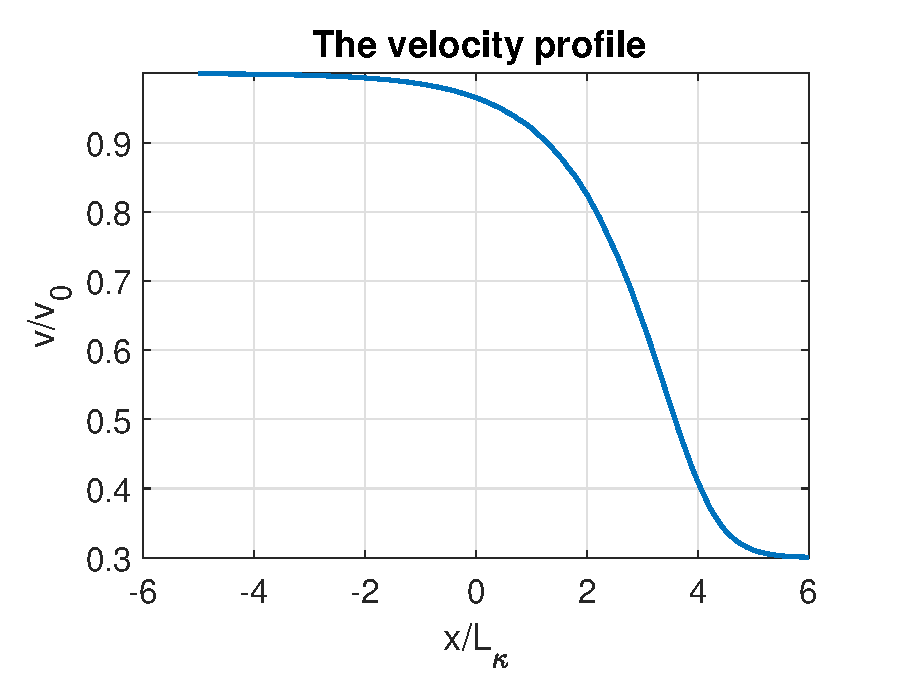
\includegraphics[width=0.8\textwidth]{1DVel.eps}
 \caption{Velocity  profile based in 1-D analytical solution.}
    \end{subfigure}%
    \begin{subfigure}[b]{0.5\textwidth}
        \centering
        \label{fig:1DTemp}
        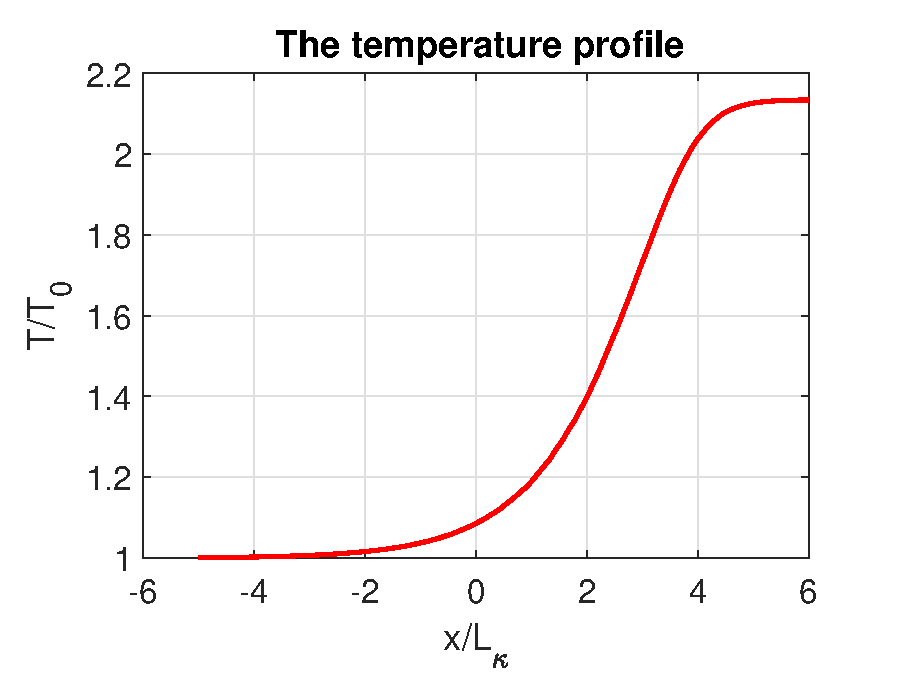
\includegraphics[width=0.8\textwidth]{1DTemp.eps}
        \caption{Temperature  profile in 1-D analytical solution.}
    \end{subfigure}
\caption{1-D Analytical solution for Large Prandtl numbers in compressible flow \cite{Johnson}}
\end{figure}
\\
As a result, for Mach number $M=1.3$, the velocity profile in figure 3.1 (a) is obtained. It shows that the velocity decreases to $30\%$ of its initial velocity. In addition, this decrease in velocity leads to amplification in temperature, the temperature reaches $220\%$ of its initial value. In real entry problem, the heat will be transferred via convection which is proportionally dependent on temperature around the rocket. The heat flux can be given as:
\begin{equation}
\label{eq:31}
\dot{Q}=hA(T_{rocket}-T_{ambient}).
\end{equation}
where $h$ is heat transfer coefficient and $A$ is the area exposed to the ambient temperature. As a result, it can be concluded that the heat transfer increases dramatically.
\begin{figure}[h!]
\label{fig:uvel}
    \centering
    \begin{subfigure}[b]{0.5\textwidth}
        \centering
        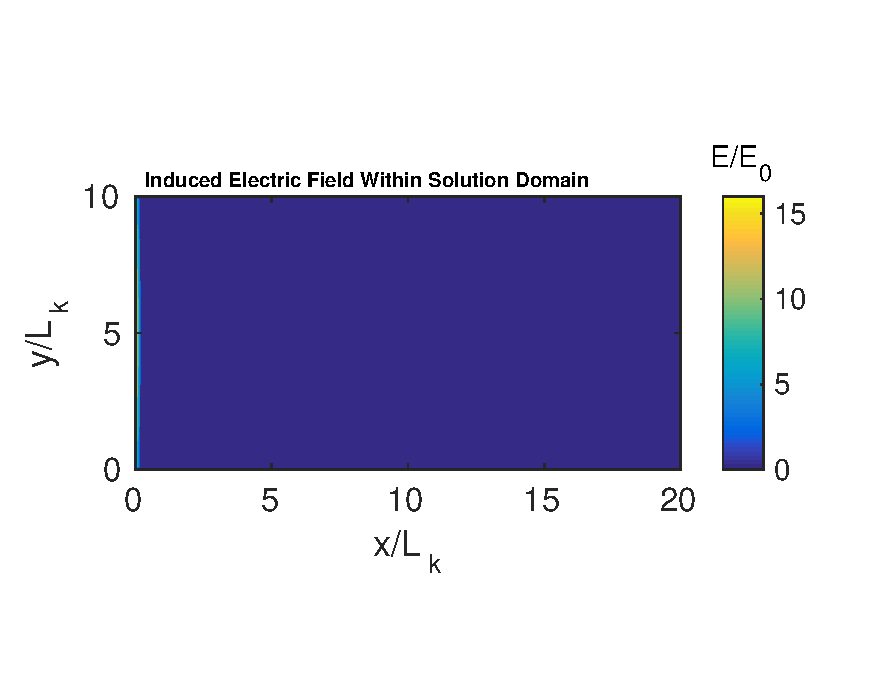
\includegraphics[width=1.\textwidth]{Ebeg.eps}
        \caption{Electric field in the beginning of the simulation}
    \end{subfigure}%
    \begin{subfigure}[b]{0.5\textwidth}
        \centering
        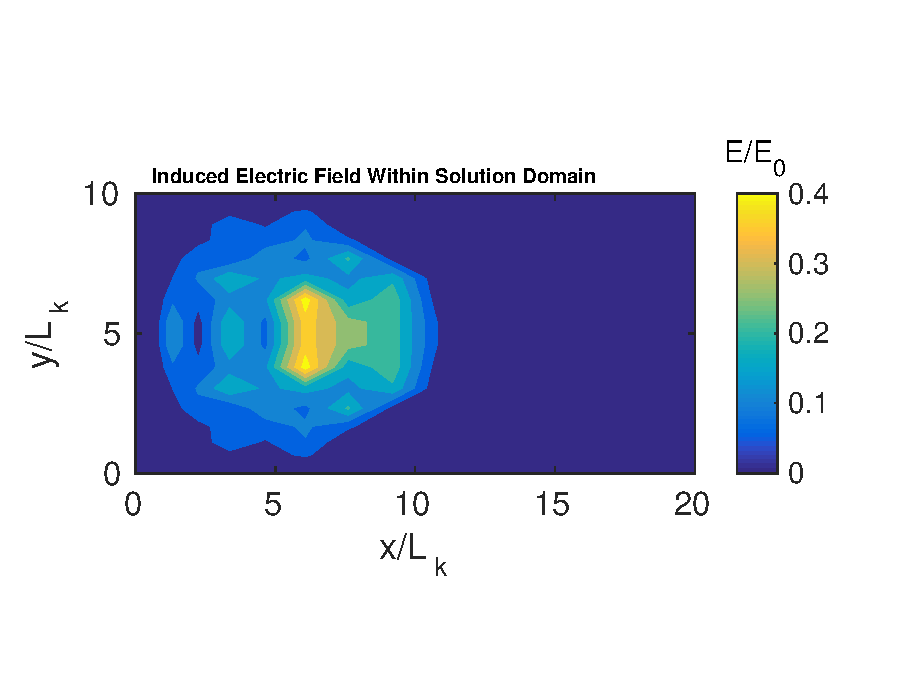
\includegraphics[width=1.\textwidth]{Emid1.eps}
        \caption{Electric field at $t=10s$,}
    \end{subfigure}
    \\
     \begin{subfigure}[b]{0.5\textwidth}
        \centering
        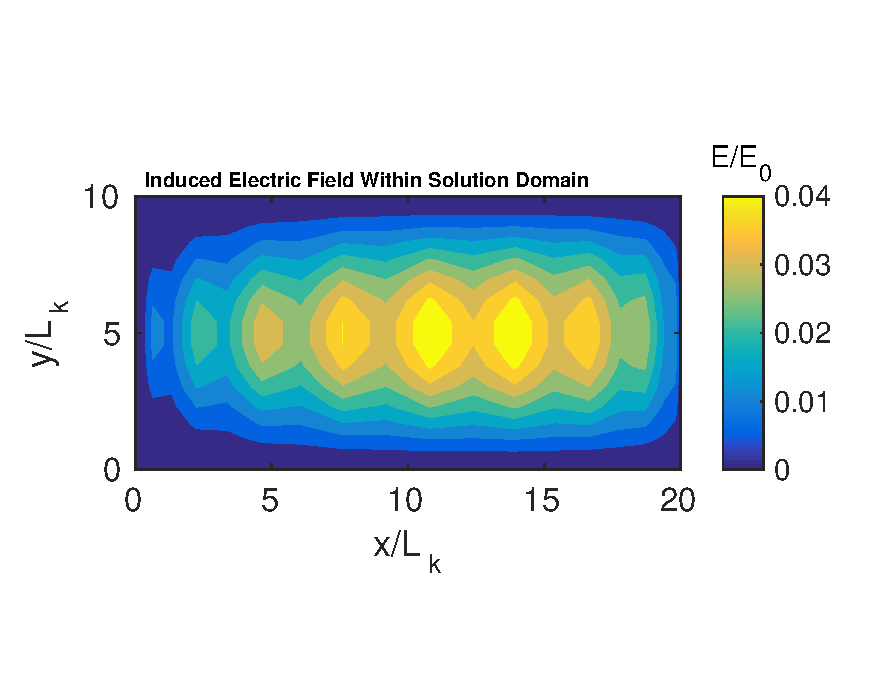
\includegraphics[width=1.\textwidth]{Emid2.eps}
        \caption{Electric field at $t=40s$}
    \end{subfigure}%
   \begin{subfigure}[b]{0.5\textwidth}
        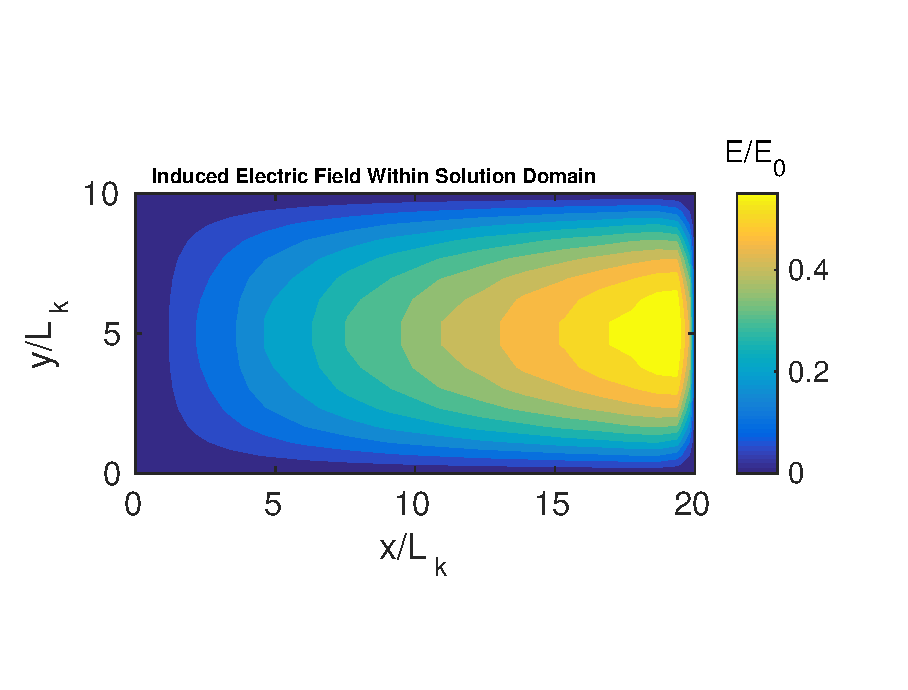
\includegraphics[width=1.\textwidth]{EFinal.eps}
        \caption{Electric field at $t=70s$}
    \end{subfigure}
    \caption{Electric field obtained at various time steps.}
\end{figure}
The presence of shock surface also affects the electric field. As the velocity decreases after shock surface, the charged particles accumulate around the solid surface this accumulation of particles also increases the charge density, therefore the electric field. In this present study, the electric field is obtained by solving set of equations given in section \ref{MHD}. Sample evolution of electric field is given in figure 3.2 at various time steps.
\chapter{Conclusion}
The atmospheric re-entry problem includes coupled effects of both compressible flow and electromagnetic effects. These effects are analysed both analytically and numerically. Briefly, the phenomena can be explained as follows. After rocket enters into atmosphere with the velocity $M>1$ , it leads to shock waves around its structure. As a result, it results in sudden temperature jumps in front of the structure which is shown analytically in figure 3.1(b). This sudden temperature increase will also enhance the heat flux towards the solid structure. In addition,  Since the charged particles accumulates in the region after shock, there is also a significant increase in electric field after shock layer. In the extended analysis, the electric field will also be coupled with the magnetic field. In real life situation, a sudden jump in electric field and magnetic will have detrimental effects on electronic components of a rocket. The results of the analysis can be used to understand these effects quantitatively. 
\\
\\
Having discussed the physical consequences of the problem, it can also be concluded that 2-D spectral element method gives accurate description of plasma flow. It provides exponential convergence as the order of Legendre polynomial increases. Moreover, since the distribution of Legendre Gauss Lobatto points are finer nearby boundaries, it gives better resolution of plasma flow. In addition, A finer mesh around the shock layer enables to get more detailed description of flow conditions.
 
\chapter{Future Work}
In this present study, a single fluid motion of plasma is analysed in 2-D setting with spectral methods. It gives fairly good results, however it is not enough to capture whole physics. First, 3-D physics is possibly different than 2-D physics, therefore a similar formulation can be extended to 3-D with spectral methods. This would produce more applicable results.
\\
\\
Moreover, currently single element is used. However, it is known that dis-continuous Galerkin\cite{Hesthaven} method is better at capturing shock surfaces. Especially, if the location of shock surface has finer mesh nearby. After forming 3-D dis-continuous Galerkin formulation, appropriate coordinate mapping will allow to extend the analysis to more realistic geometries. 
 \\
 \\
 Last but not least, the analysis performed here is done under continuum assumption. It is a very good assumption in most cases, however it may not give accurate results in Ionosphere as ions are rarefied in this layer of atmosphere. Thus including statistical models such as Vlasov equations\cite{IntPlasma} may give more accurate results for the problem analysed here.

\appendix

\chapter{Spectral Methods}
\section{ Differentiation Matrix \label{Diff}}
The differentiation matrix on Legendre-Gauss-Lobatto(GLL) points can be given as:
\begin{equation}
\label{eq:100}
D_{ij}=
\left\{\begin{matrix}
if(i=j=1 ) & \frac{1}{4}N(N-1)\\ 
if(i=j=N) & \frac{1}{4}N(N-1) \\ 
if(i=j) & 0\\ 
else &  \frac{L_i}{L_j \times (x_i - x_j)}
\end{matrix}\right.
\end{equation}
where $L_i$ and $L_j$ are Legendre polynomials defined on GLL grid points.

\section{Spectral Filtering \label{Filter}}
Spectral filtering applied in this present study is done in finite Legendre transformed data, On our GLL grid with $N+1$ points, $N_{th}$ order Legendre polynomial can be used, therefore each function represented on these grid points can be represented in terms of $N_{th}$ order Legendre polynomials as:
\begin{equation}
\label{eq:110}
f(x)\approx \hat{f}(x)= \sum_{i=0}^{N}\alpha_i P_i(x).
\end{equation}
The idea is to similar to Fourier transform, the function $\hat{f}(x)$ is multiplied with $P_i(x)$ and integrated from $-1$ to $1$ which is the mother interval of Legendre polynomials. Since Legendre polynomials are mutually orthogonal to each other, the right hand side of equation \ref{eq:110} reduces to a single term. The inner product of Legendre polynomial by itself is already given in equation \ref{eq:32}, therefore the result of integration can be given as:
\begin{equation}
\label{eq:111}
\sum_{j=1}^{N}\hat{f}(x_j)P_i(x_j)w_j=\frac{2 \alpha_i}{2+i}
\end{equation}
where $x_j$ is GLL grid points. Therefore, the coefficients of Legendre polynomials are given as:
\begin{equation}
\label{eq:112}
\alpha_i=\frac{(2+i)\times \sum_{j=1}^{N}\hat{f}(x_j)P_i(x_j)w_j}{2}
\end{equation}
However, the function $f(x)$ may be oscillating with very high wave number so that it may not be represented in the grid chosen. Therefore high frequency terms build up on coefficients $\alpha_i$. It is called aliasing error\cite{Hesthaven}. This aliasing error tend to accumulate at higher coefficients whereas the value we try to represent are at first coefficients. Therefore, These coefficients can be filtered to avoid aliasing error. The filter function is defined as:
\begin{equation}
H(i)=\exp(-(\frac{i}{\sigma})^p).
\end{equation}
where $p$ is the order of the filter function and $\sigma$ is the half length of the filter function. This function is multiplied with the corresponding coefficients, therefore the filter coefficients are obtained as:
\begin{equation}
\label{eq:113}
\hat{\alpha}_i=H(i)\alpha_i=\exp(-(\frac{i}{\sigma})^p)\alpha_i.
\end{equation}
These coefficients are multiplied with the corresponding Legendre polynomial To obtain the filtered function:
\begin{equation}
\label{eq:114}
\tilde{f}(x)=\sum_{i=0}^{N}\hat{\alpha}_i P_i(x).
\end{equation}
This filtering operation will enable to ensure stability of time integration in non-linear time dependent problems.
\section{Weak Formulation \label{Weak}}
As a first example of weak formulation, heat equation in 1-D can be used as it has diffusive property:
\begin{equation}
\label{eq:130}
u_t=u_{xx}.
\end{equation}
Moreover, $u$ can be written in terms of Legendre polynomials as follows:
\begin{equation}
\label{eq:131}
u=\sum_{i=1}^{N_x}\alpha_{i}(t) P_i(x)
\end{equation}
where $\alpha_i$ is the corresponding coefficient of a Legendre polynomial and $N_x$ is the order of Legendre polynomials used. If the spectral decomposition \ref{eq:131} is replaced back into equation \ref{eq:130}, the following equation is obtained:
\begin{equation}
\label{eq:132}
\sum_{i=1}^{N_x}\dot{\alpha_{i}} P_i=\sum_{i=1}^{N_x}\alpha_{i} {P}''_i
\end{equation}
If the equation \ref{eq:132} is multiplied with $P_j$ which is a Legendre polynomial at $j_{th}$ order and integrated over whole domain, the following form equation is obtained:
\begin{equation}
\label{eq:133}
\sum_{j=1}^{N_x}\sum_{i=1}^{N_x}\dot{\alpha_{i}} P_i P_j w_i =\sum_{j=1}^{N_x} \sum_{i=1}^{N_x}\alpha_{i} {P}''_i P_j w_i.
\end{equation}
By the functional orthogonality of Legendre polynomials, left hand side of equation \ref{eq:133} reduces to the mass matrix. Moreover, using integration by part, right hand side of equation can also be represented in terms of first derivative products of Legendre polynomials. As a result, the following equation is obtained:
\begin{equation}
\label{eq:134}
\dot{\alpha_{j}}  w_j=- \sum_{i=1}^{N_x}\alpha_{i} {P}'_i {P}'_j w_i
\end{equation}
In matrix form, equation \ref{eq:134} can be given as:
\begin{equation}
\label{eq:135}
[\mathbf{M}]\dot{\alpha}=[\mathbf{K}]\alpha.
\end{equation}
where $[\mathbf{M}]$ is a diagonal mass matrix with diagonal entries $w_j$ and $[\mathbf{K}]$ is the stiffness matrix which is a full matrix. 
\chapter{Matlab Routines}
\section{1-D Analytical Shock Solver}
\lstinputlisting{AnalyticalShock.m} 
\lstinputlisting{getClosedFormShock.m} 
\lstinputlisting{getShockVelocity.m} 


\bibliographystyle{plain}
\bibliography{mybib}% Produces the bibliography via BibTeX.

\end{document}
